% Options for packages loaded elsewhere
\PassOptionsToPackage{unicode}{hyperref}
\PassOptionsToPackage{hyphens}{url}
%
\documentclass[
]{article}
\usepackage{lmodern}
\usepackage{amssymb,amsmath}
\usepackage{ifxetex,ifluatex}
\ifnum 0\ifxetex 1\fi\ifluatex 1\fi=0 % if pdftex
  \usepackage[T1]{fontenc}
  \usepackage[utf8]{inputenc}
  \usepackage{textcomp} % provide euro and other symbols
\else % if luatex or xetex
  \usepackage{unicode-math}
  \defaultfontfeatures{Scale=MatchLowercase}
  \defaultfontfeatures[\rmfamily]{Ligatures=TeX,Scale=1}
\fi
% Use upquote if available, for straight quotes in verbatim environments
\IfFileExists{upquote.sty}{\usepackage{upquote}}{}
\IfFileExists{microtype.sty}{% use microtype if available
  \usepackage[]{microtype}
  \UseMicrotypeSet[protrusion]{basicmath} % disable protrusion for tt fonts
}{}
\makeatletter
\@ifundefined{KOMAClassName}{% if non-KOMA class
  \IfFileExists{parskip.sty}{%
    \usepackage{parskip}
  }{% else
    \setlength{\parindent}{0pt}
    \setlength{\parskip}{6pt plus 2pt minus 1pt}}
}{% if KOMA class
  \KOMAoptions{parskip=half}}
\makeatother
\usepackage{xcolor}
\IfFileExists{xurl.sty}{\usepackage{xurl}}{} % add URL line breaks if available
\IfFileExists{bookmark.sty}{\usepackage{bookmark}}{\usepackage{hyperref}}
\hypersetup{
  pdftitle={GMACwriteup2.RMD},
  pdfauthor={Jarred Kvamme, University of Idaho},
  hidelinks,
  pdfcreator={LaTeX via pandoc}}
\urlstyle{same} % disable monospaced font for URLs
\usepackage[margin=1in]{geometry}
\usepackage{graphicx,grffile}
\makeatletter
\def\maxwidth{\ifdim\Gin@nat@width>\linewidth\linewidth\else\Gin@nat@width\fi}
\def\maxheight{\ifdim\Gin@nat@height>\textheight\textheight\else\Gin@nat@height\fi}
\makeatother
% Scale images if necessary, so that they will not overflow the page
% margins by default, and it is still possible to overwrite the defaults
% using explicit options in \includegraphics[width, height, ...]{}
\setkeys{Gin}{width=\maxwidth,height=\maxheight,keepaspectratio}
% Set default figure placement to htbp
\makeatletter
\def\fps@figure{htbp}
\makeatother
\setlength{\emergencystretch}{3em} % prevent overfull lines
\providecommand{\tightlist}{%
  \setlength{\itemsep}{0pt}\setlength{\parskip}{0pt}}
\setcounter{secnumdepth}{-\maxdimen} % remove section numbering

\title{GMACwriteup2.RMD}
\author{Jarred Kvamme, University of Idaho}
\date{9/22/2021}

\begin{document}
\maketitle

\hypertarget{variance-across-tissues-plots}{%
\subsection{variance across tissues
plots}\label{variance-across-tissues-plots}}

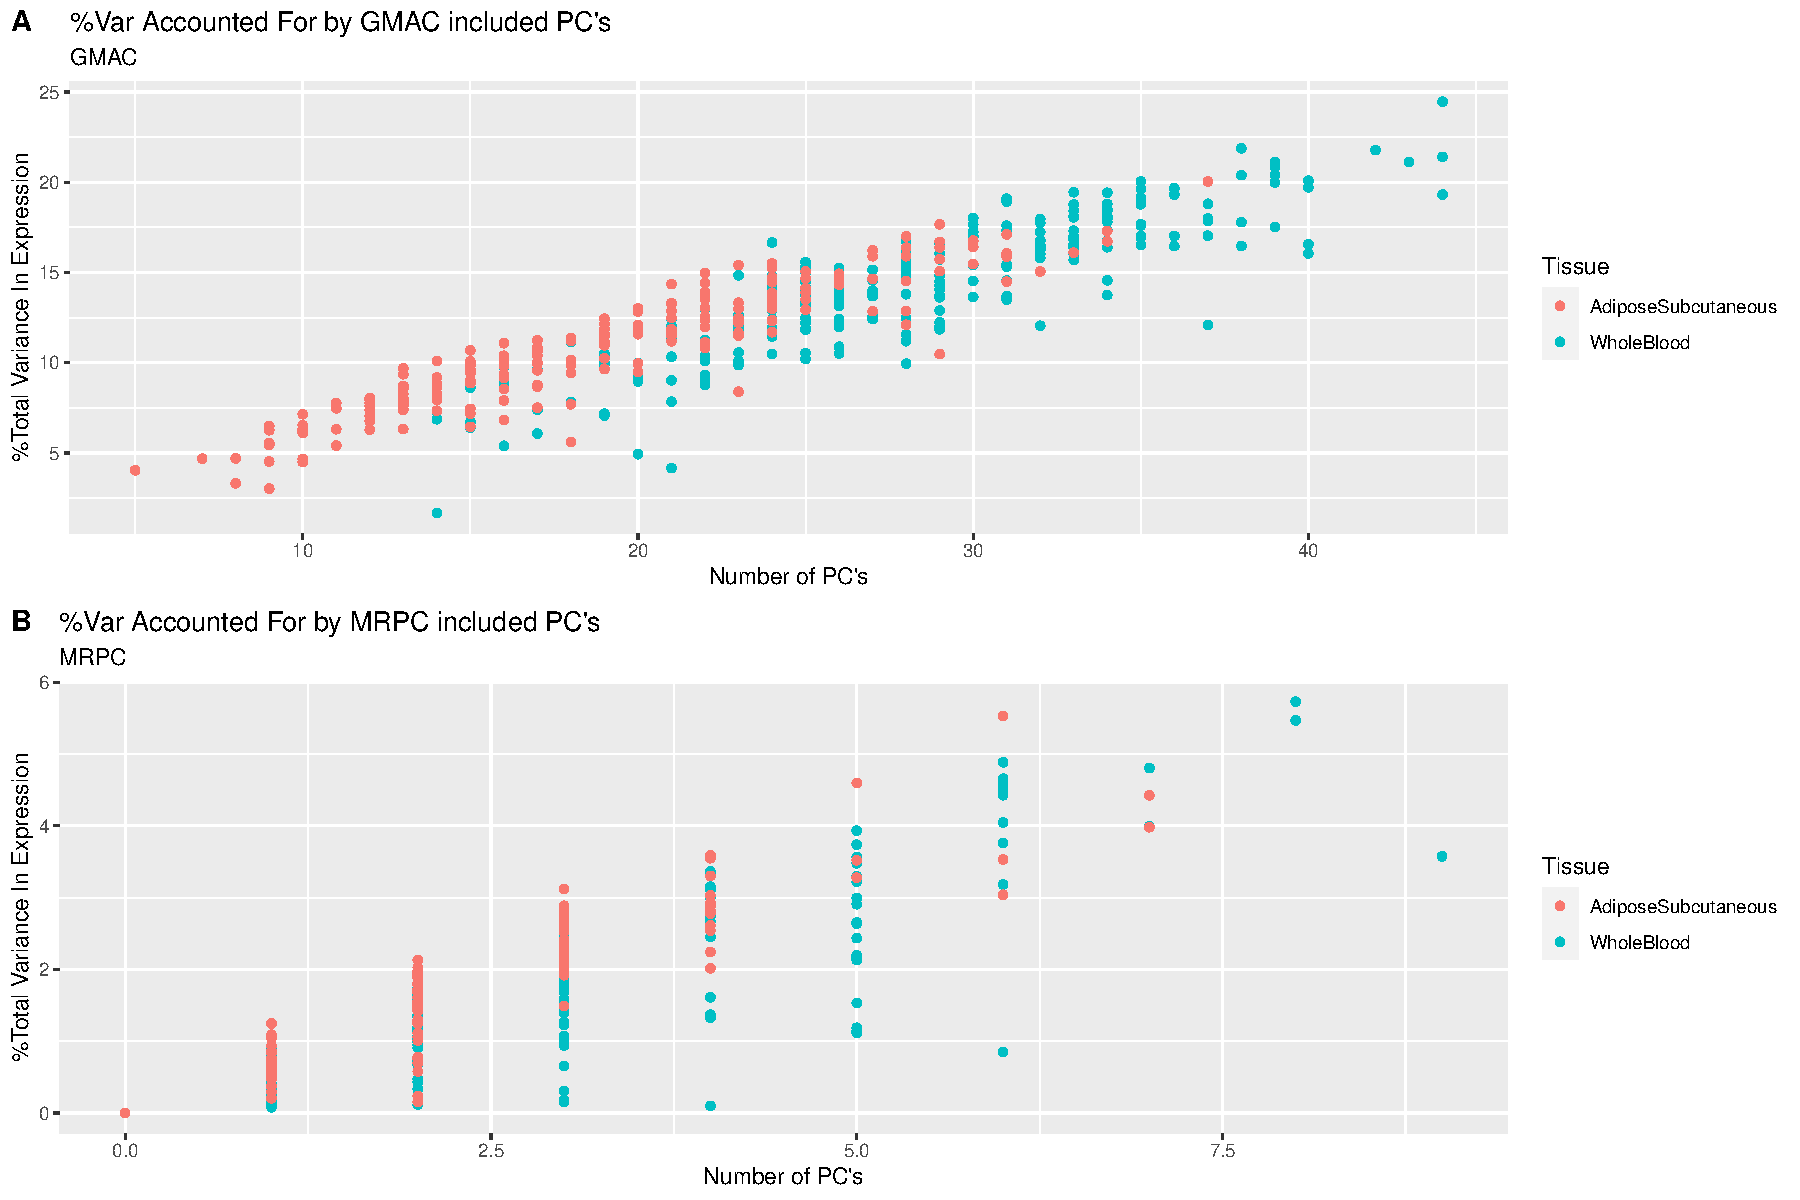
\includegraphics{GMACwriteup2_files/figure-latex/unnamed-chunk-1-1.pdf}

\hypertarget{ltm-and-stm-plots}{%
\subsection{LTM and STM plots}\label{ltm-and-stm-plots}}

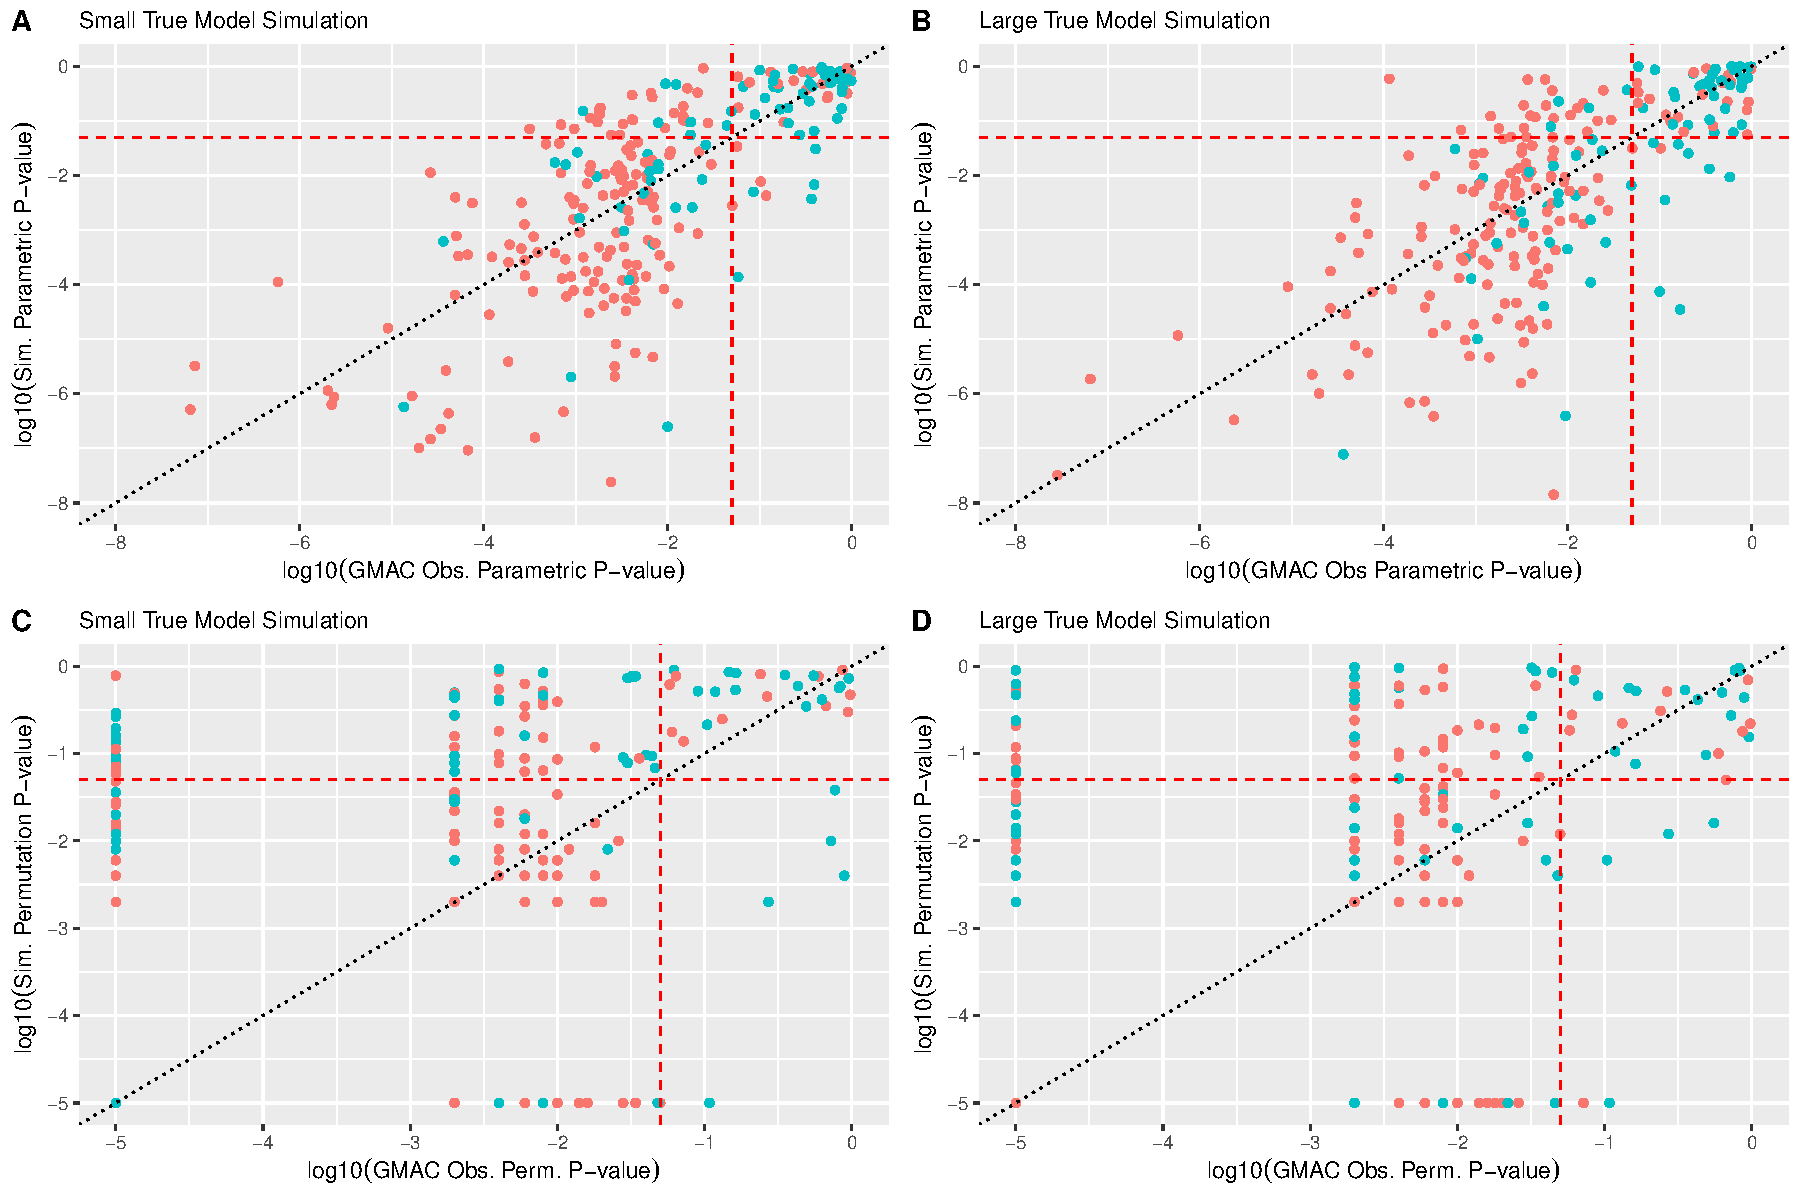
\includegraphics{GMACwriteup2_files/figure-latex/unnamed-chunk-2-1.pdf}

\hypertarget{tgm-and-mrpc-plots}{%
\subsection{TGM and MRPC plots}\label{tgm-and-mrpc-plots}}

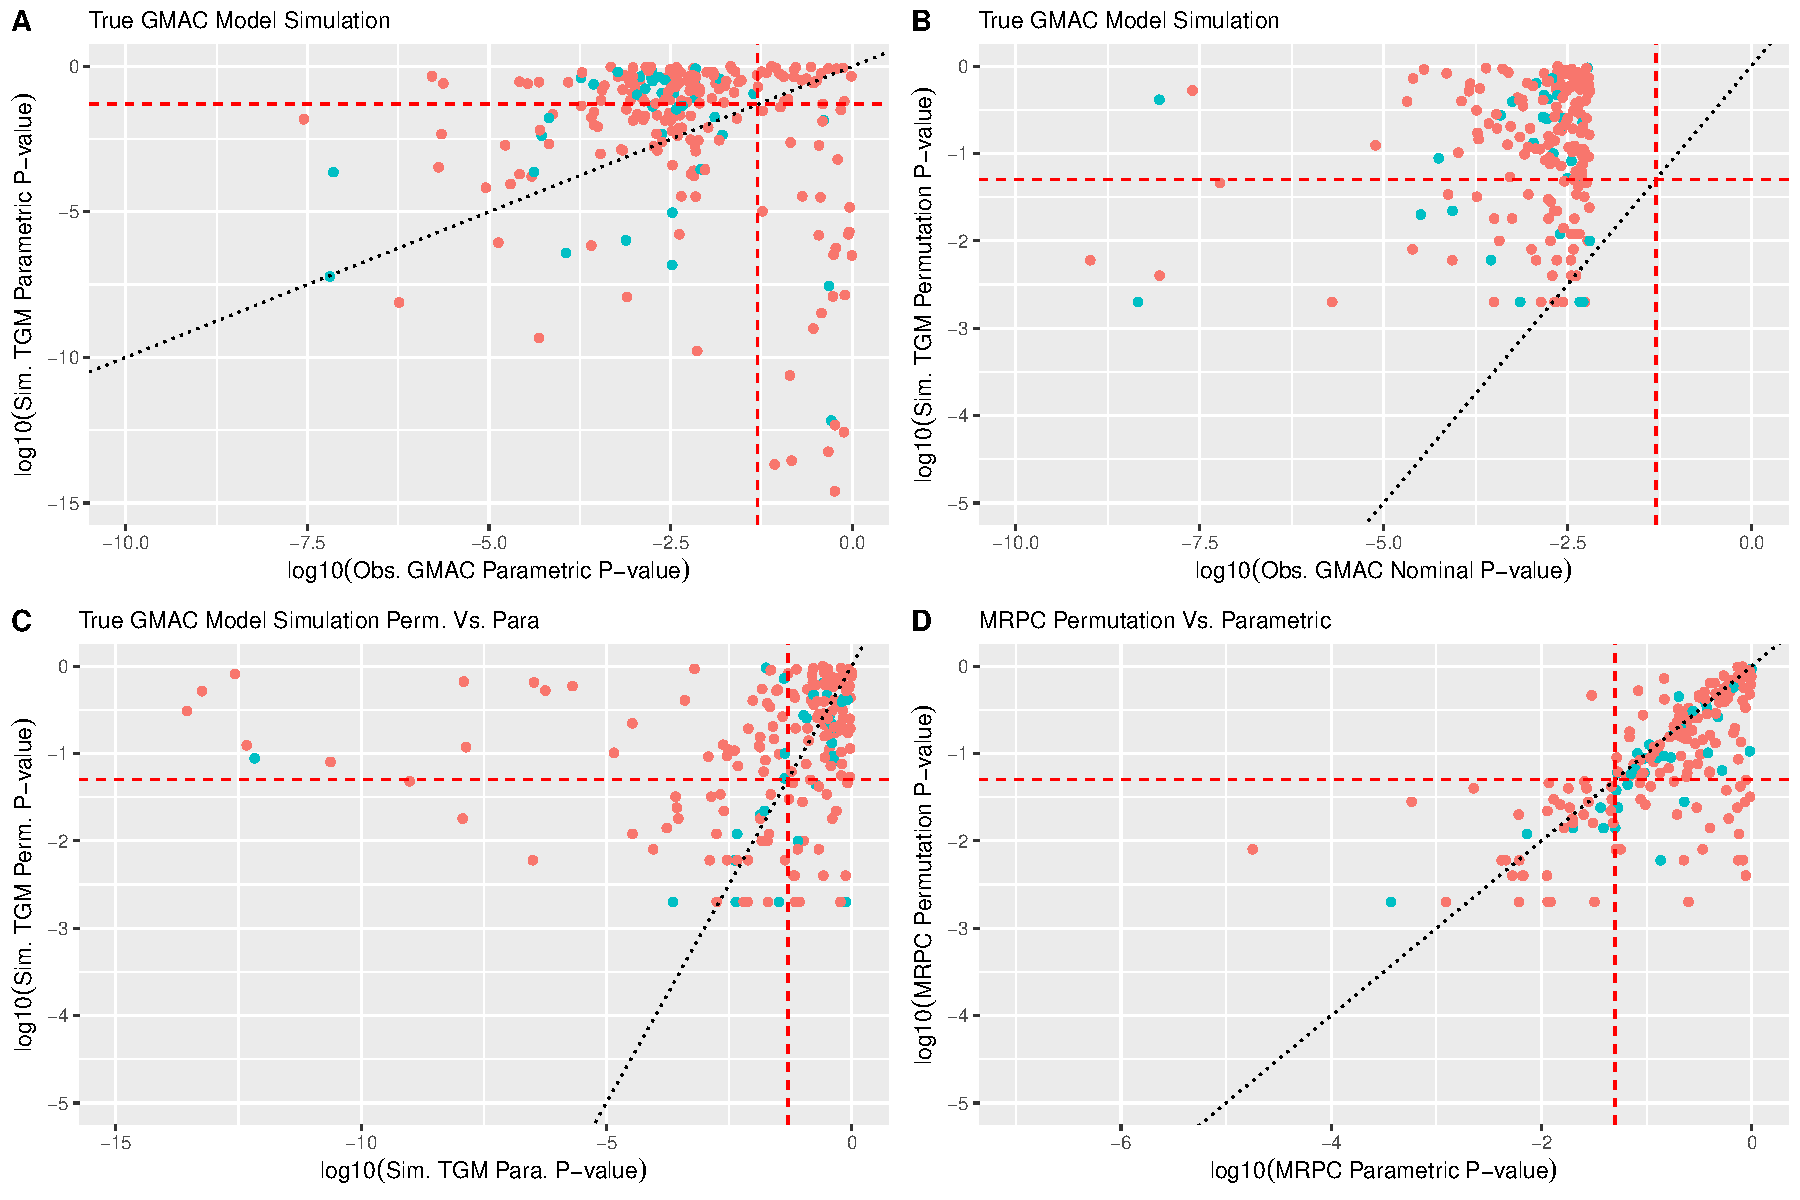
\includegraphics{GMACwriteup2_files/figure-latex/unnamed-chunk-3-1.pdf}

\hypertarget{gss-and-gmac-plots}{%
\subsection{GSS and GMAC plots}\label{gss-and-gmac-plots}}

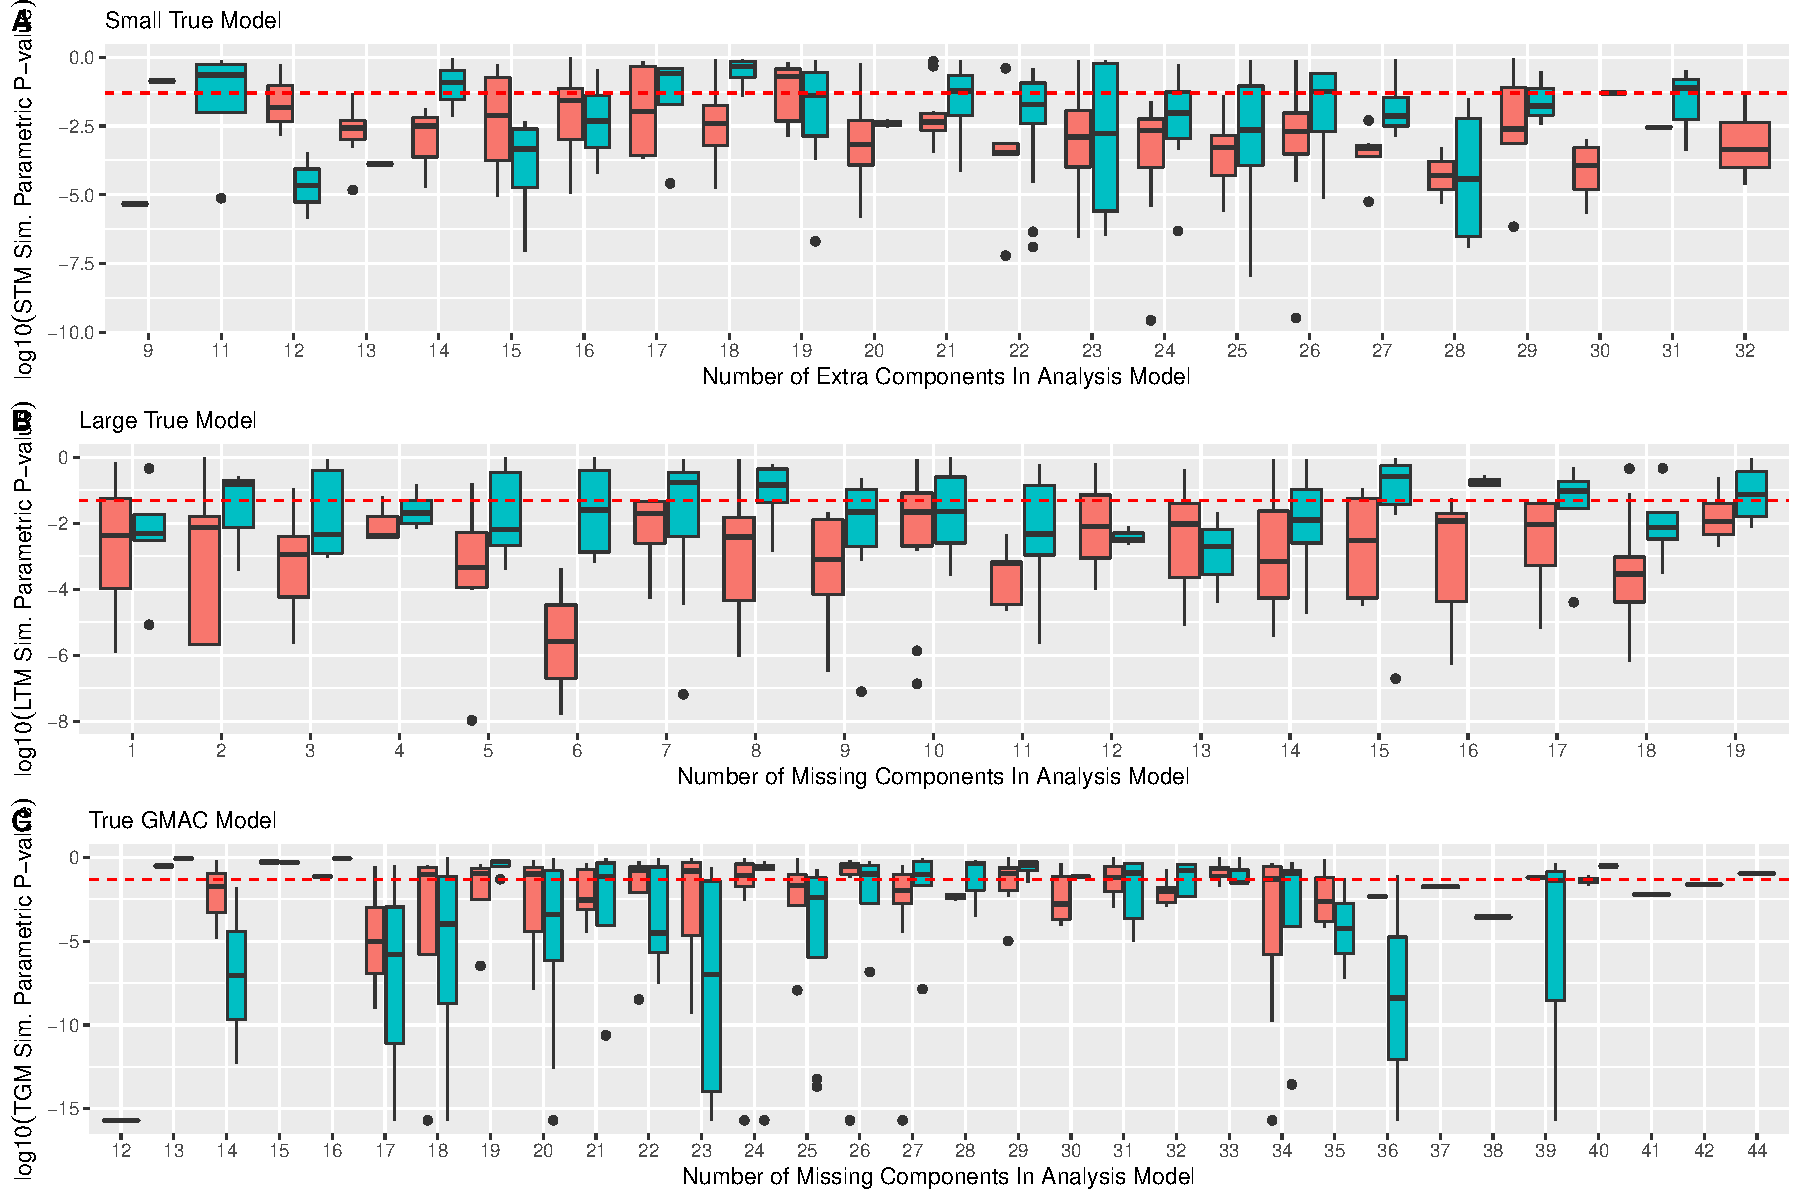
\includegraphics{GMACwriteup2_files/figure-latex/unnamed-chunk-4-1.pdf}

\hypertarget{nominal-p-value-plots}{%
\subsection{Nominal P-value plots}\label{nominal-p-value-plots}}

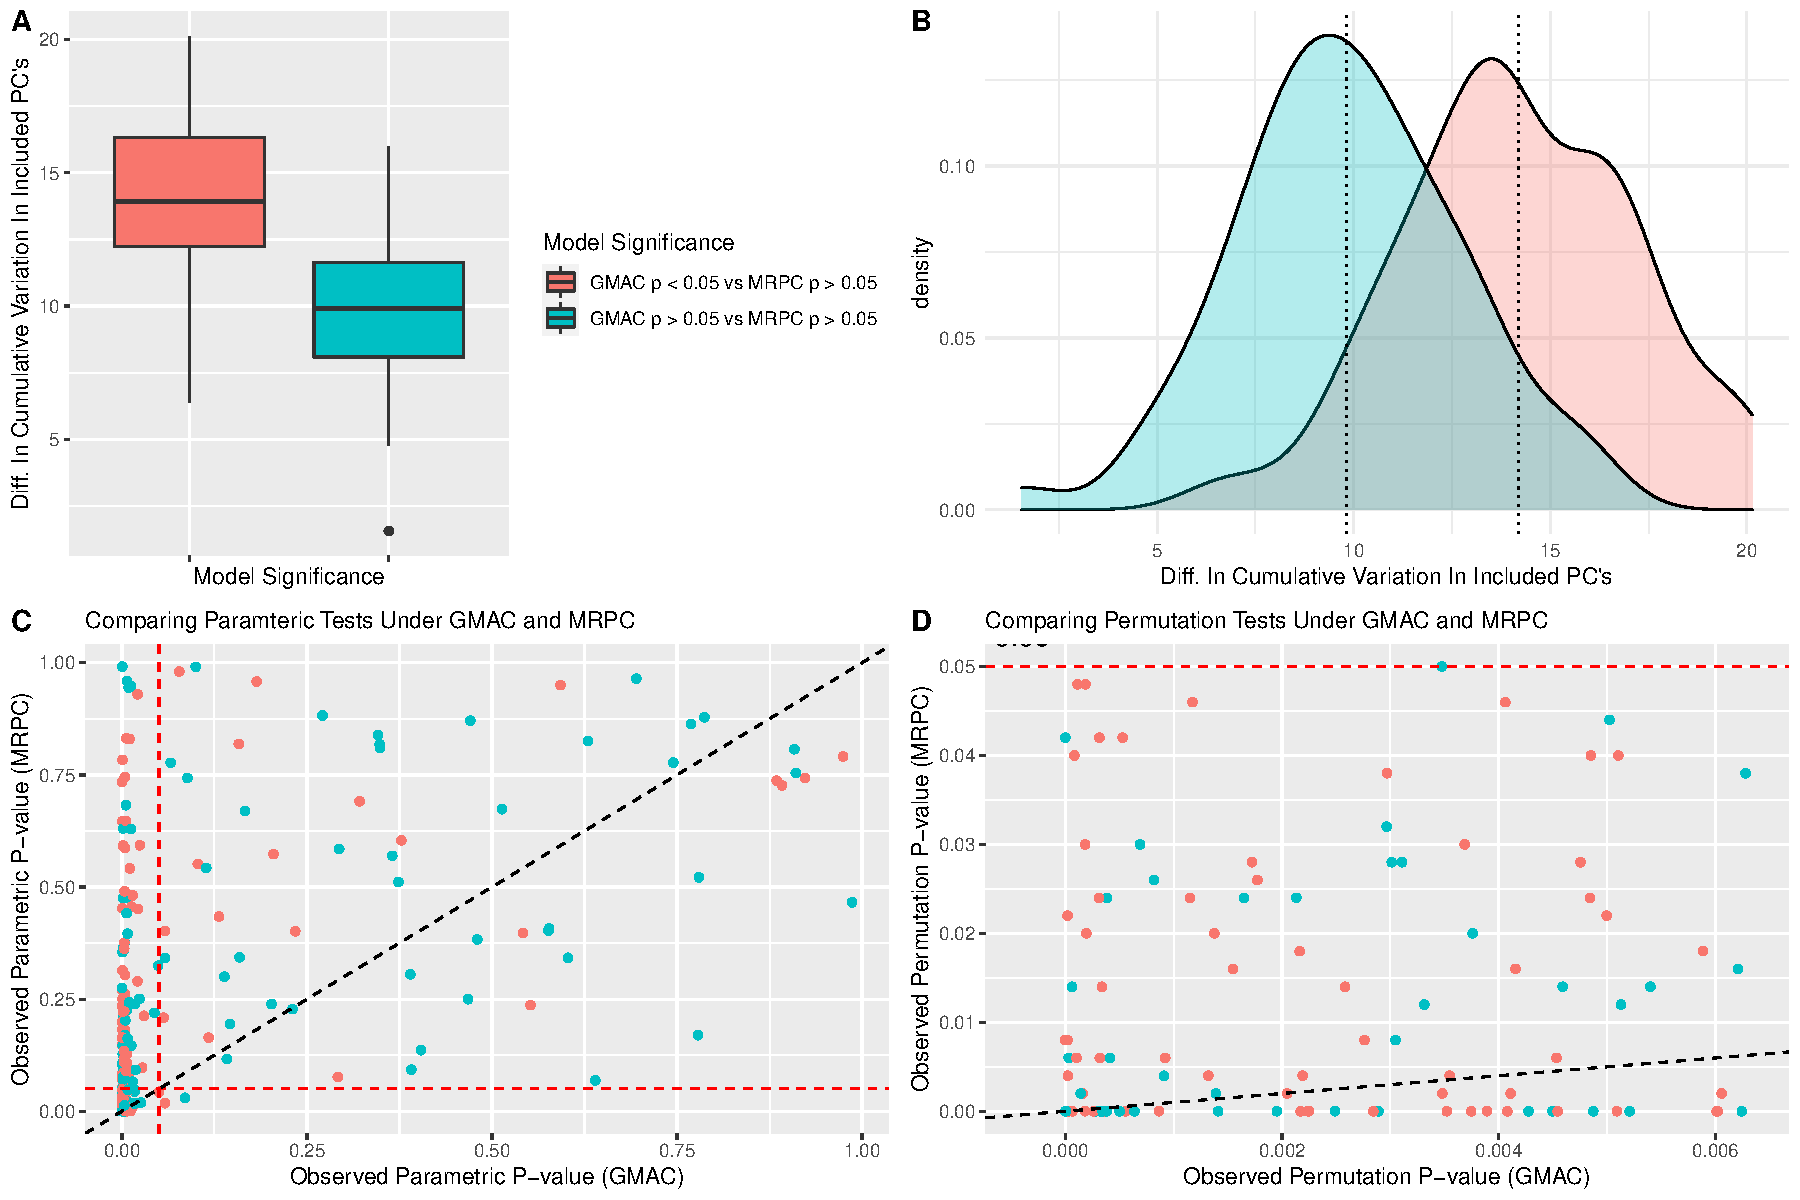
\includegraphics{GMACwriteup2_files/figure-latex/unnamed-chunk-5-1.pdf}

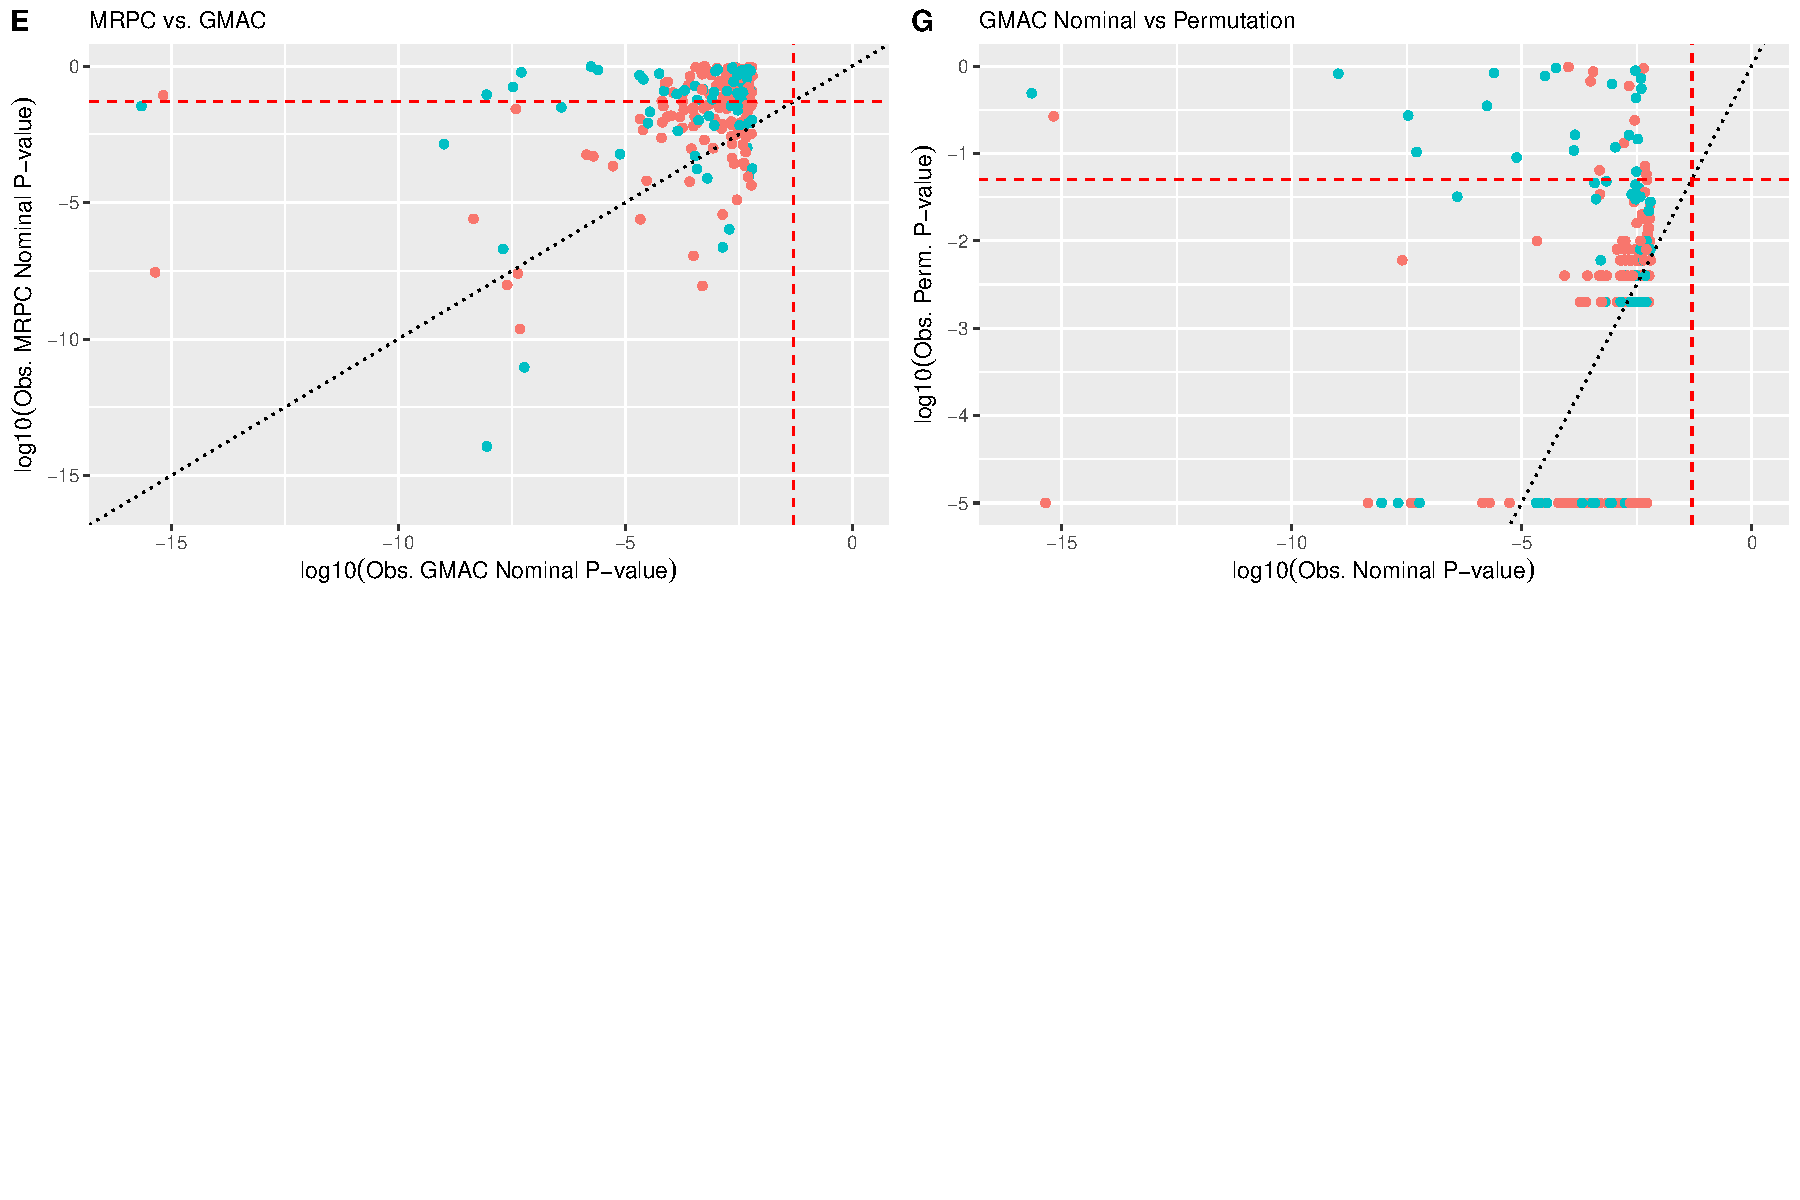
\includegraphics{GMACwriteup2_files/figure-latex/unnamed-chunk-6-1.pdf}

\hypertarget{boxplots-for-pc-inclusion-differences}{%
\subsection{boxplots for PC inclusion
differences}\label{boxplots-for-pc-inclusion-differences}}

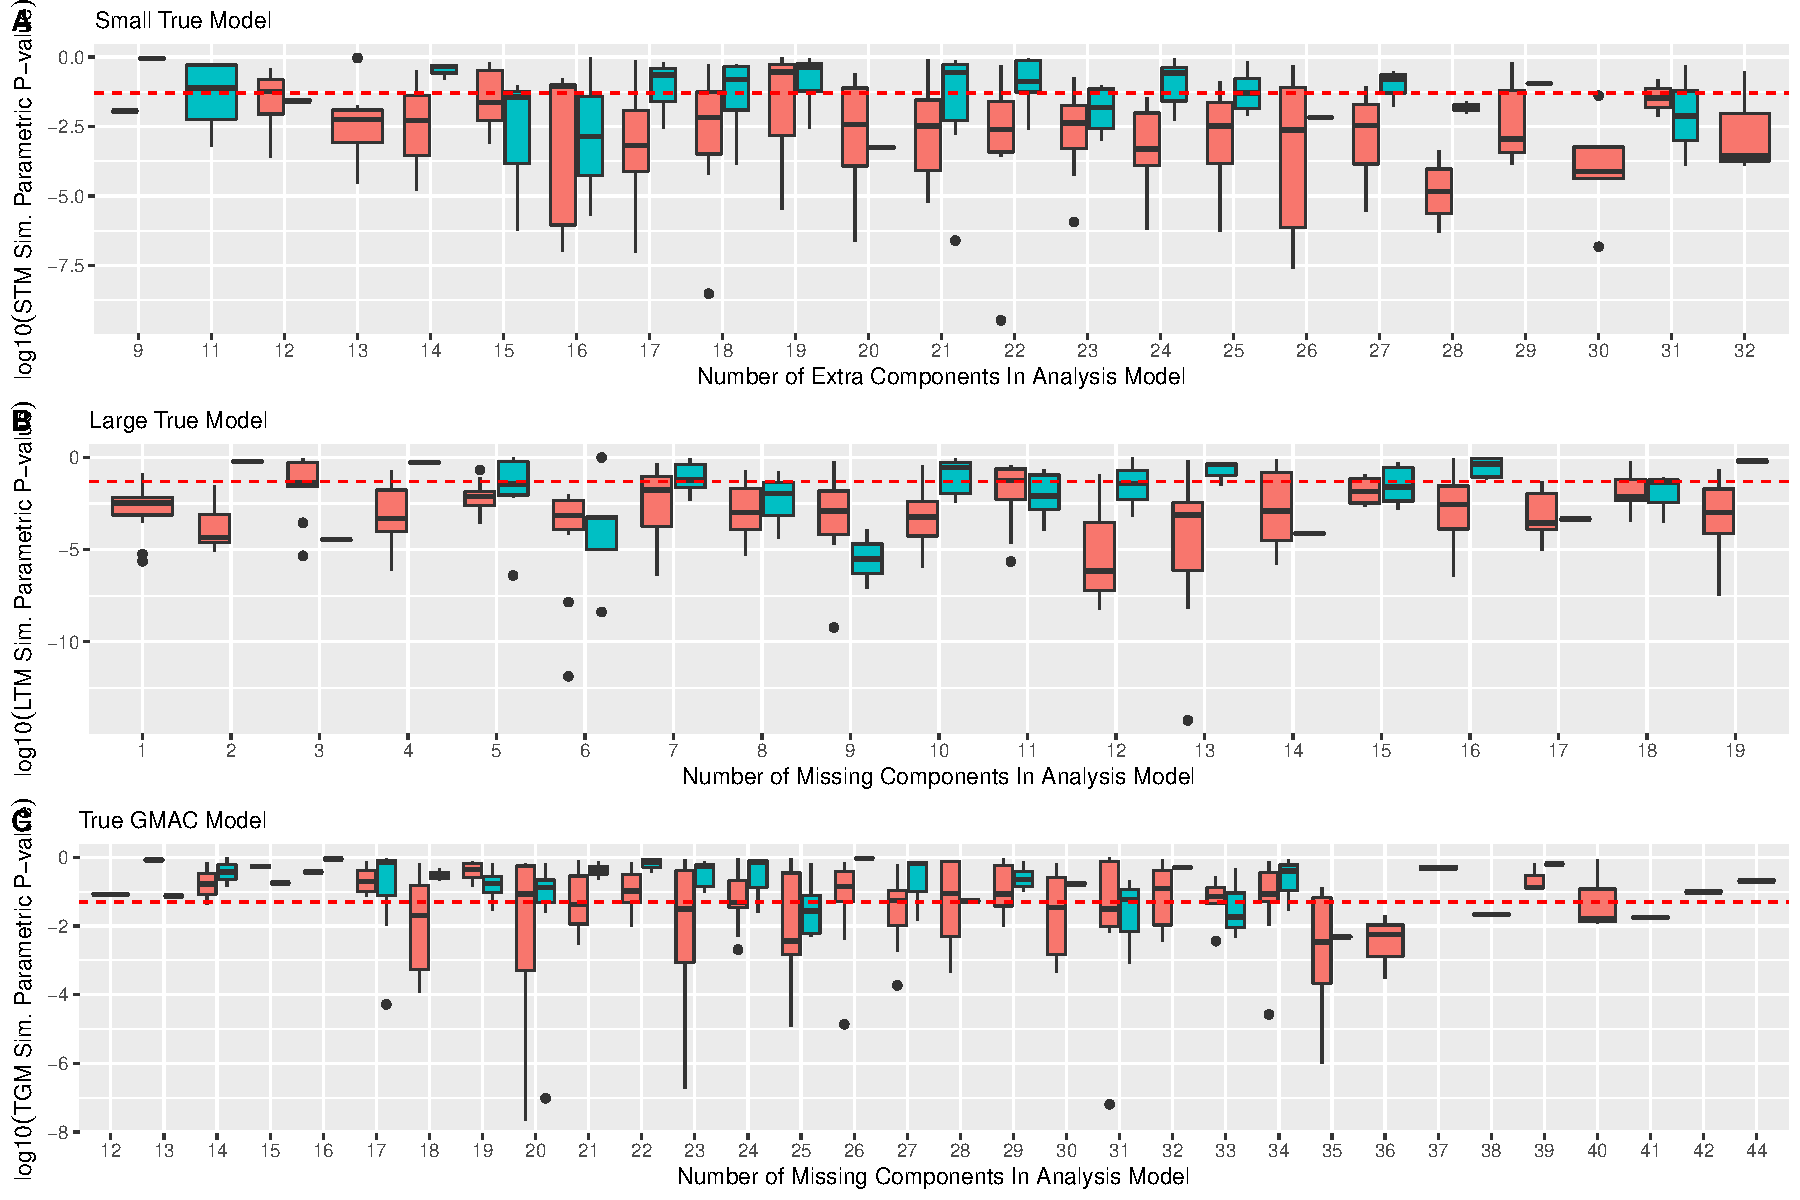
\includegraphics{GMACwriteup2_files/figure-latex/unnamed-chunk-7-1.pdf}

\hypertarget{variation-differences-between-sig-and-non-sig-trios-gmacmrpc}{%
\subsection{variation differences between sig and non-sig trios
GMAC/MRPC}\label{variation-differences-between-sig-and-non-sig-trios-gmacmrpc}}

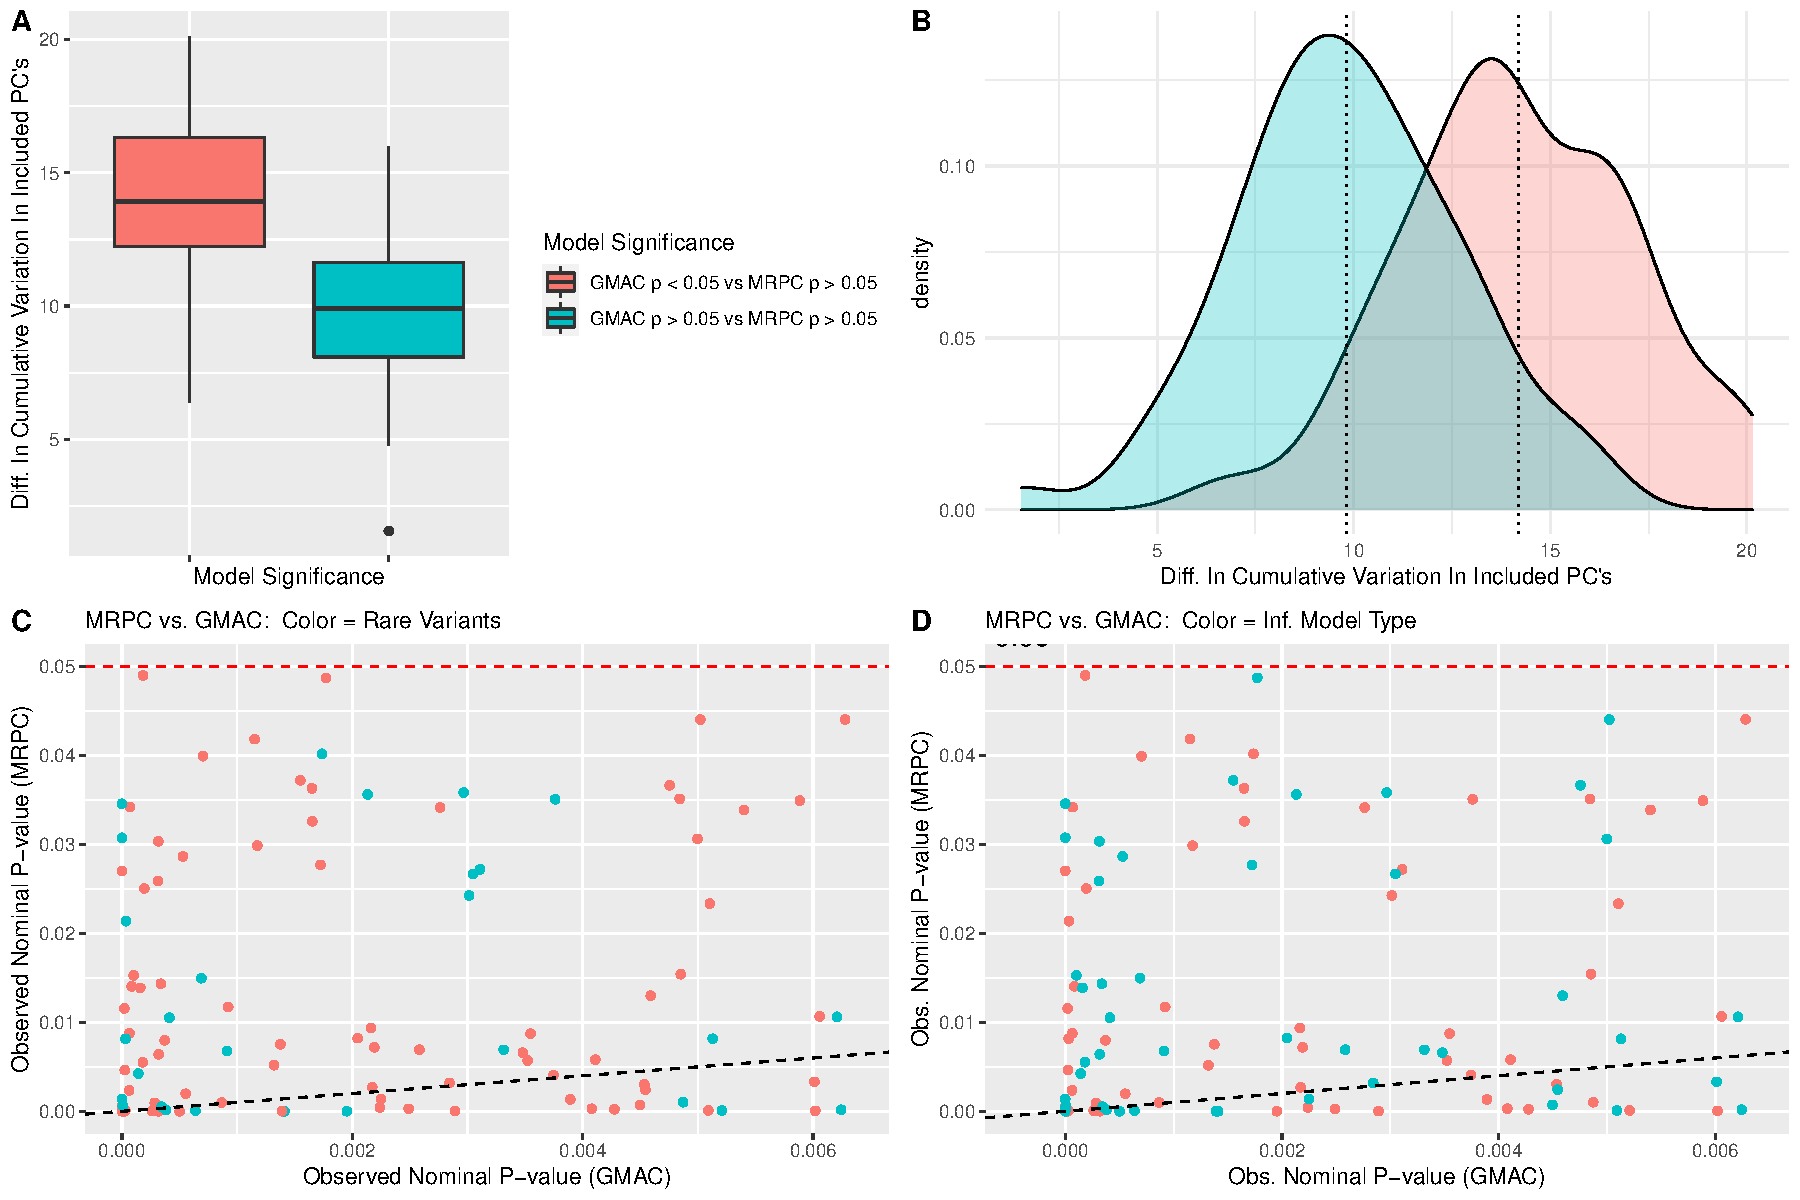
\includegraphics{GMACwriteup2_files/figure-latex/unnamed-chunk-8-1.pdf}

\end{document}
